\section{Overview}

In this chapter it will be described the Implementation, Integration, and Test Plan for the S\&C application. The aim is to ensure that the system is built incrementally, with a focus on reliability, modularity, and ease of testing.

The implementation and integration of the S\&C application will adopt a \textbf{Bottom-Up strategy}. This method begins by focusing on the foundational components located at the lower levels of the uses hierarchy. These modules are the smallest units of functionality that do not depend on other modules. Each module will be tested using dedicated drivers to ensure correctness and reliability before being integrated into the larger system.

As modules are validated, they will replace the corresponding drivers and be incrementally integrated into functional subsystems. This iterative process ensures that each subsystem is tested and functional before further integration. The Bottom-Up strategy facilitates parallel development, allowing different teams to work on separate modules simultaneously, and simplifies debugging by isolating issues within smaller parts of the system.

This strategy promotes incremental progress, enabling the early detection of bugs and providing stakeholders with visible milestones throughout the development process. The result is a robust and well-tested system that meets the application's requirements.

\section{Implementation plan}

The implementation plan follows a \textbf{Bottom-Up} approach, starting with foundational elements and progressing toward more complex components and user-facing services. Each stage builds on the previous one, ensuring a stable foundation for the subsequent layers and modules. This structured approach ensures that all dependencies are resolved before higher-level functionalities are developed.

\begin{enumerate}
    \item
\textbf{Database Management System (DBMS):} \\
The first step is the implementation of the Database Management System (DBMS), which serves as the foundation of the system.

\begin{figure}[H]
    \centering
    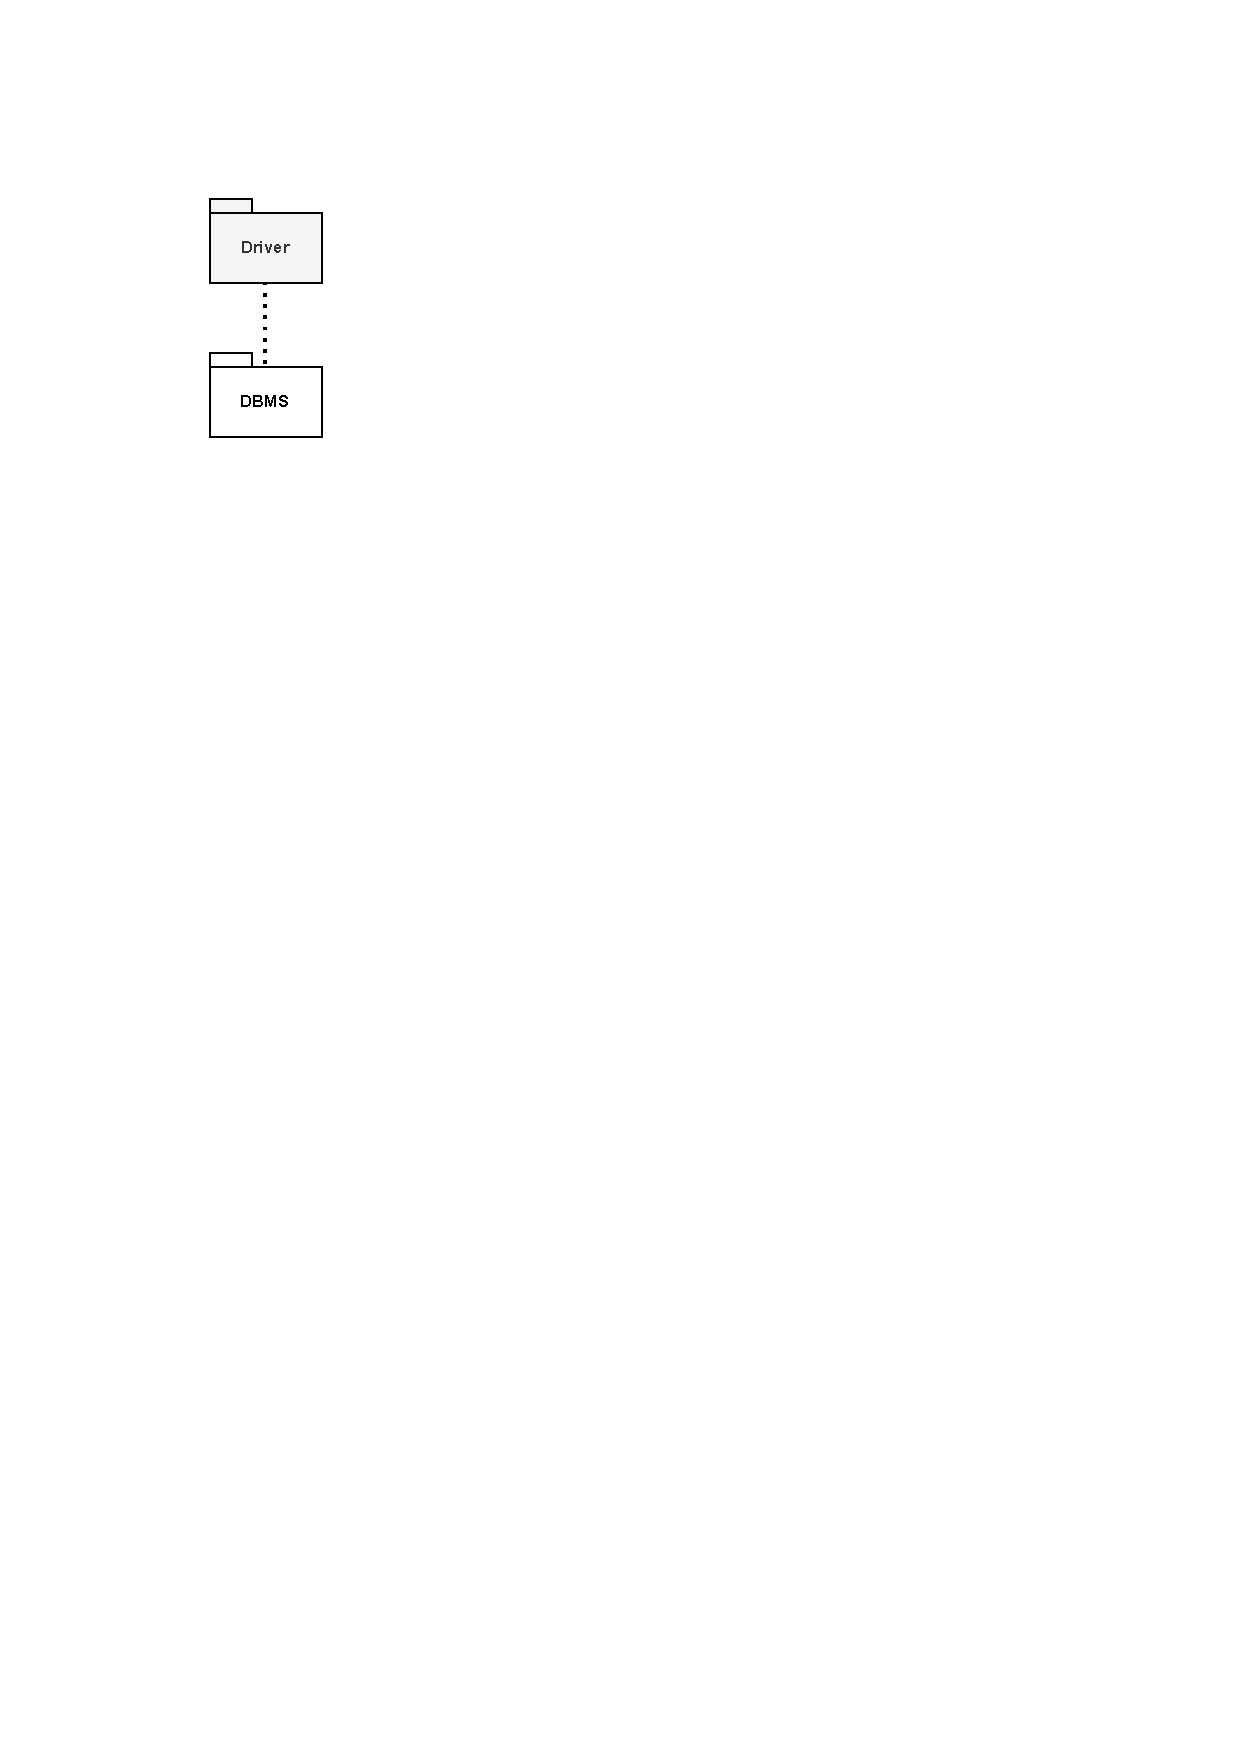
\includegraphics[width=0.25\linewidth]{DD/Images/Testing/1_DBMS.pdf}
    \caption{Integration 1: DBMS.}
    \label{fig:integration_1}
\end{figure}

Starting with the database ensures that all components relying on persistent data storage (e.g., Account Manager, Internship Manager) have a consistent and reliable backend.
    \item
\textbf{Authentication Services (Authentication Manager in Account Manager):} \\
Once the DBMS is ready, the next step is implementing the Authentication Manager.

\begin{figure}[H]
    \centering
    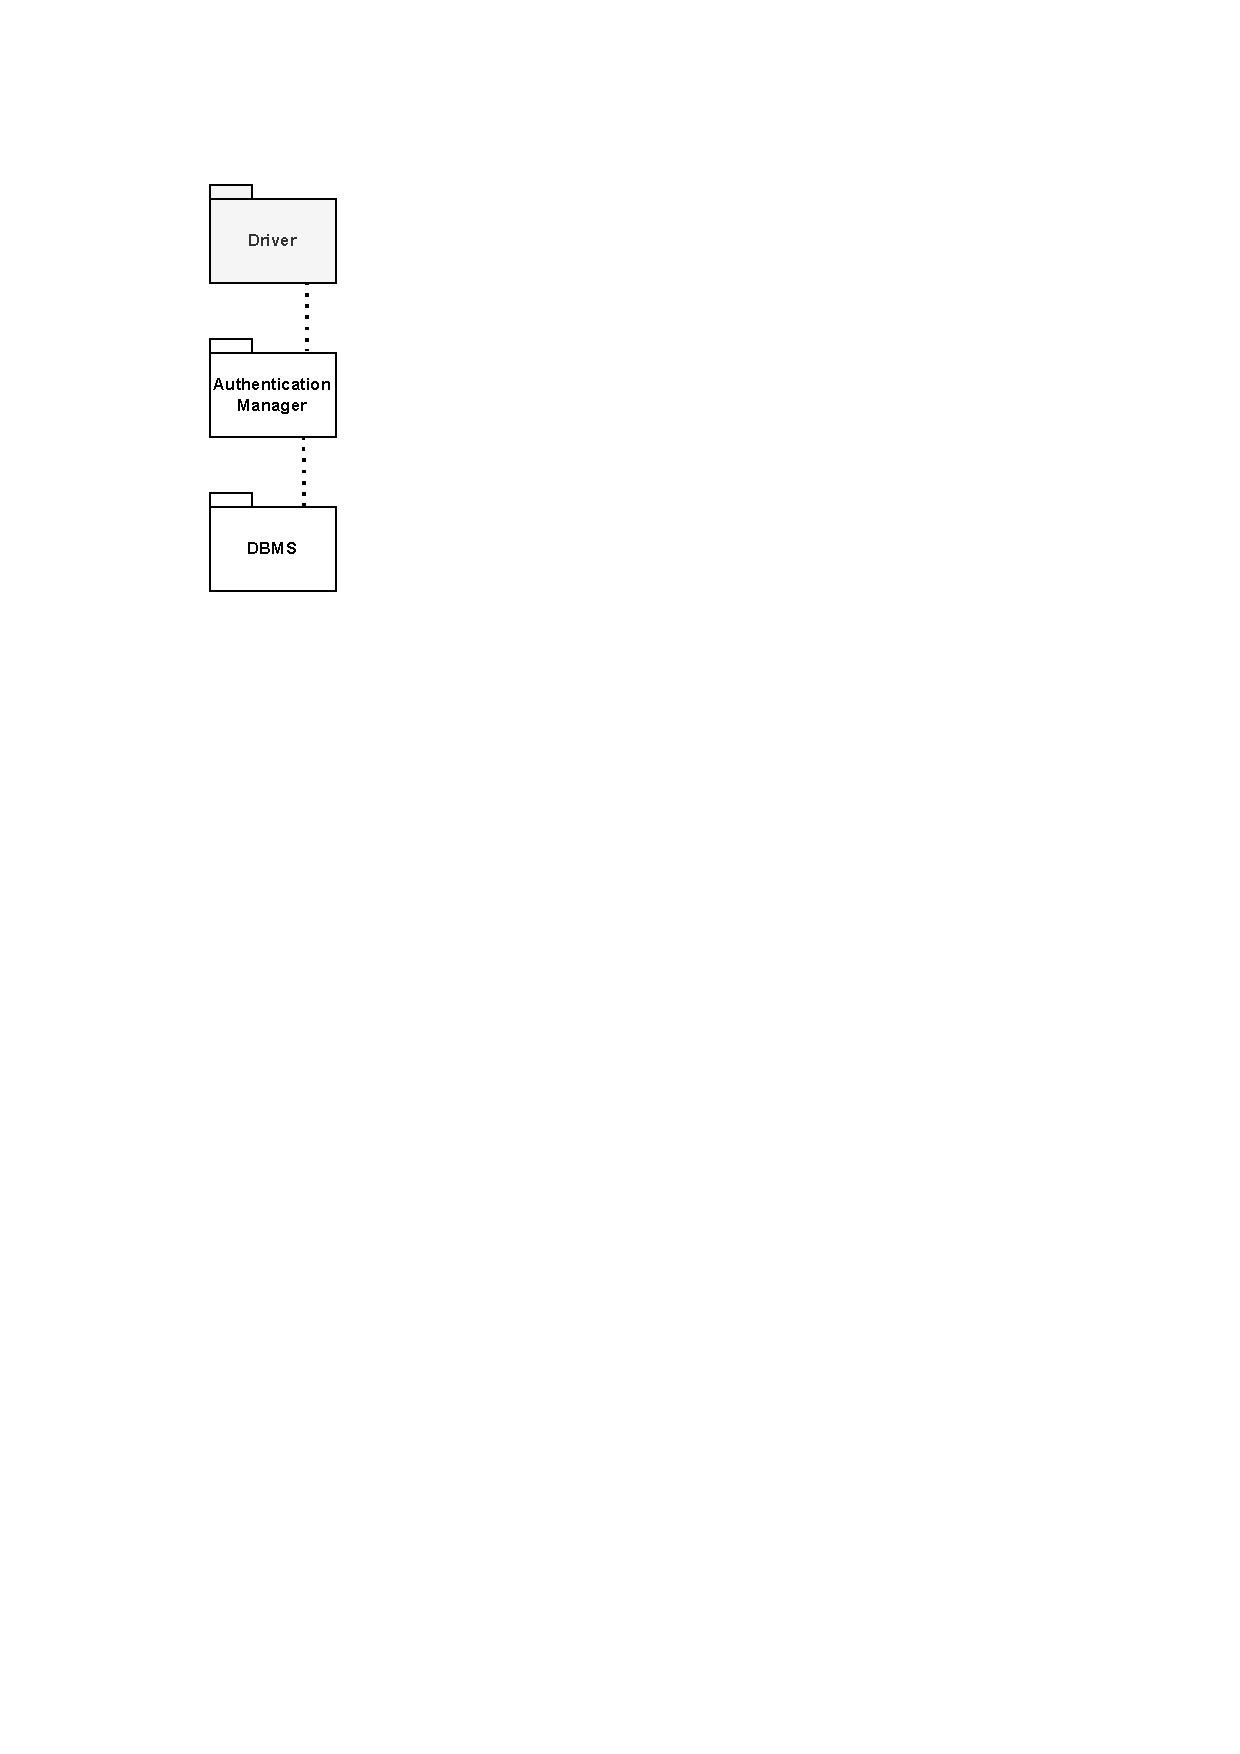
\includegraphics[width=0.3\linewidth]{DD/Images/Testing/2_auth.pdf}
    \caption{Integration 2: Authentication Manager.}
    \label{fig:integration_2}
\end{figure}

The Authentication Manager is foundational for controlling access to the system. Its successful implementation ensures that subsequent components can rely on secure user identification and role management.
    \item
\textbf{Registration Services (Registration Managers in Account Manager):} \\
The next step is developing the Registration Services, which handle the creation of new user accounts.

\begin{figure}[H]
    \centering
    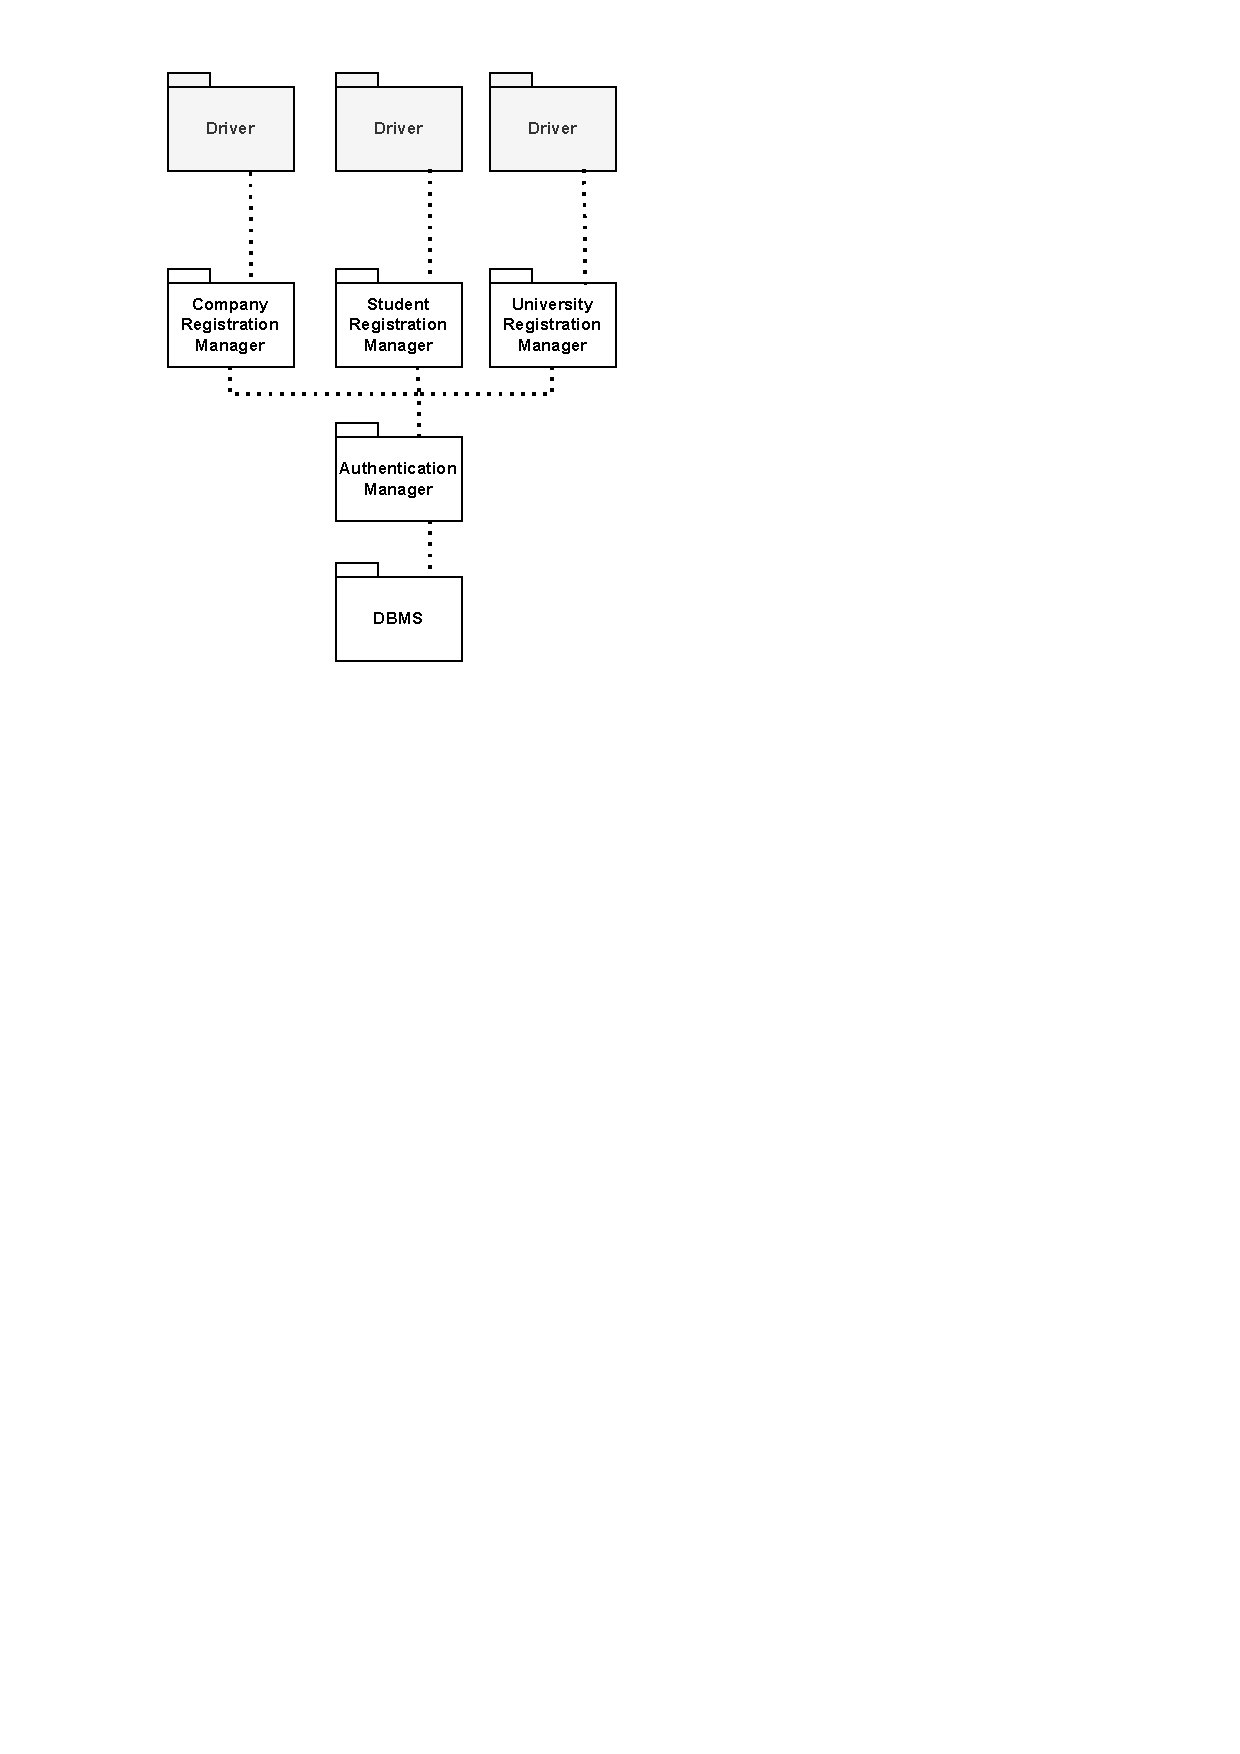
\includegraphics[width=0.5\linewidth]{DD/Images/Testing/3_reg.pdf}
    \caption{Integration 3: Registration Managers.}
    \label{fig:integration_3}
\end{figure}

Registration Services depend on both the database and authentication systems. Completing these ensures that users can securely create accounts before managing profiles or accessing the system.
\newpage
    \item 
\textbf{Account Features (Account Updater in Account Manager):} \\
The Account Updater handles profile management for all users.

\begin{figure}[H]
    \centering
    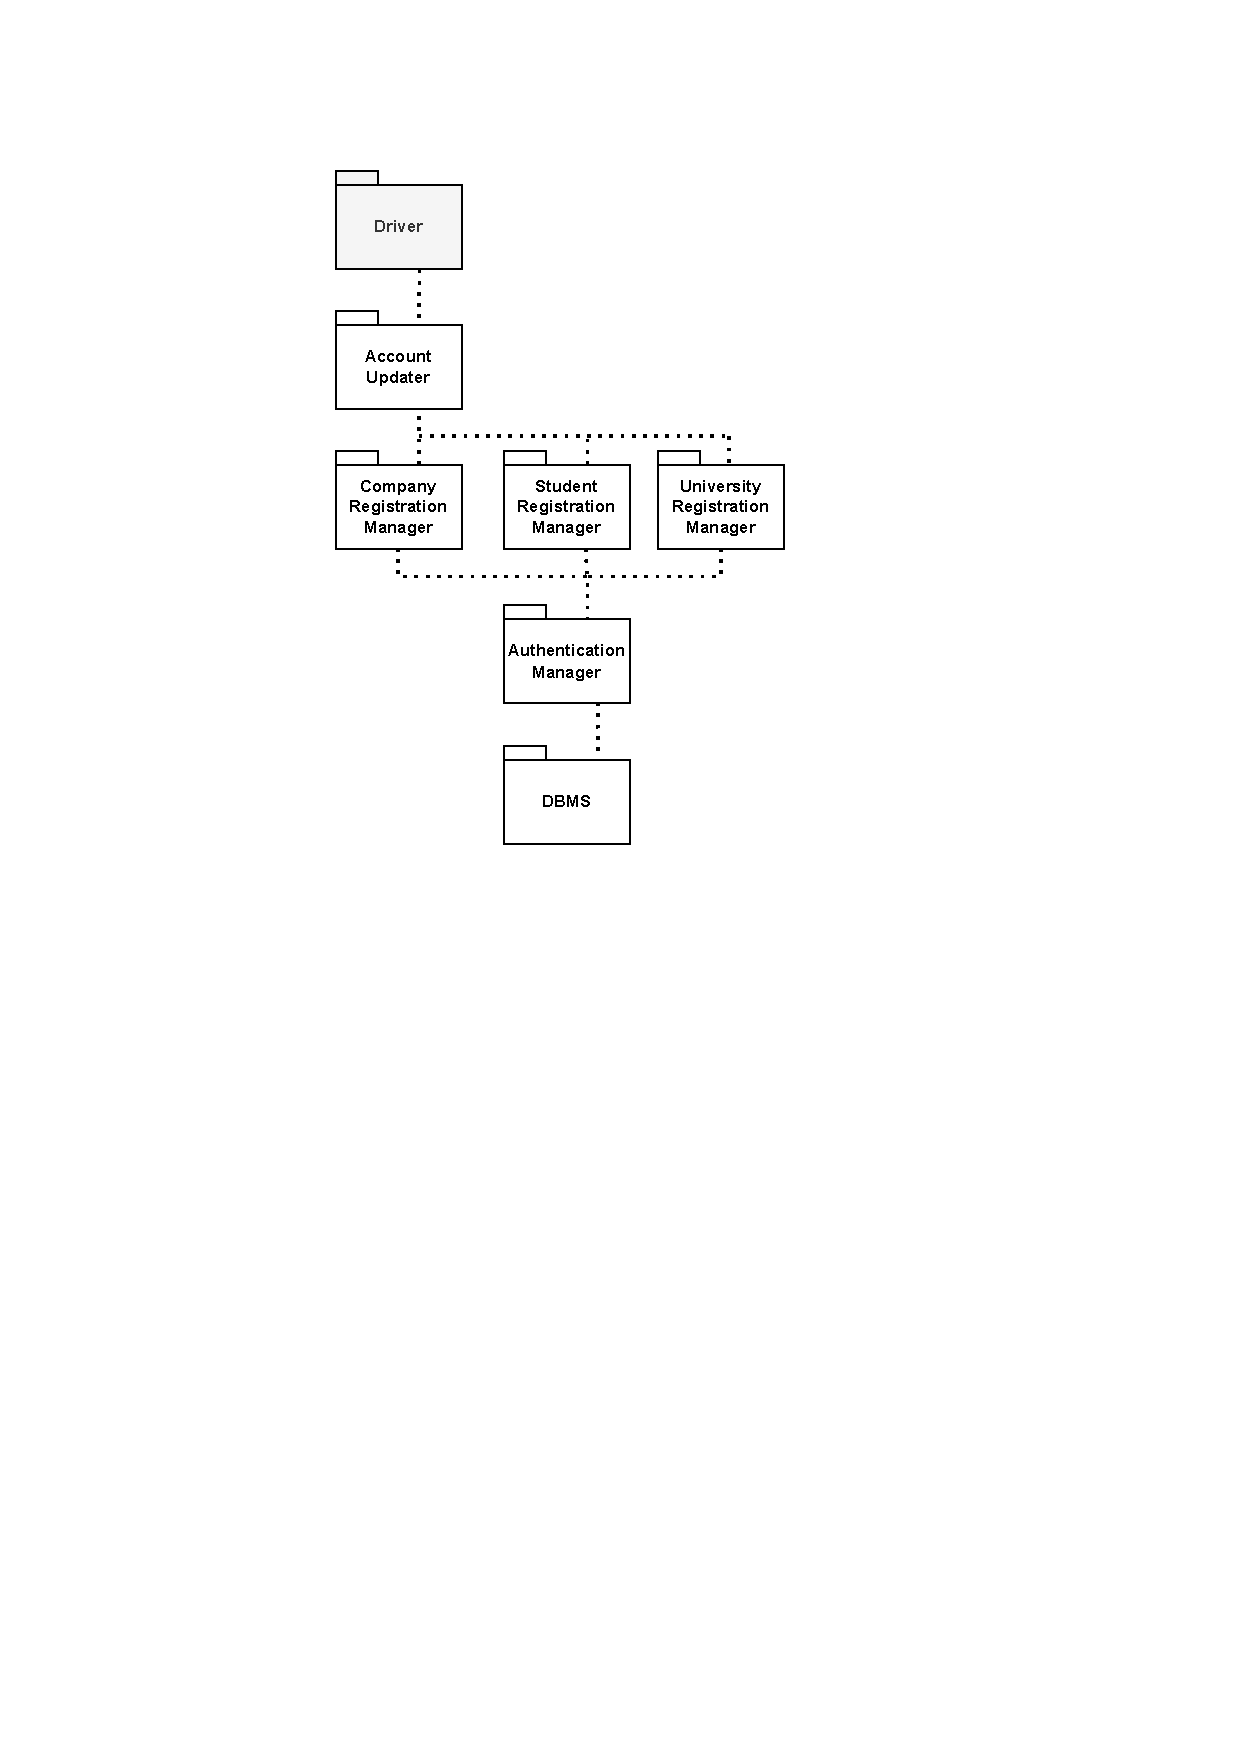
\includegraphics[width=0.5\linewidth]{DD/Images/Testing/4_AccUpdater.drawio.pdf}
    \caption{Integration 4: Account Updater.}
    \label{fig:integration_4}
\end{figure}

Building the Account Updater after the Authentication and Registration Services ensures that all user actions are authenticated and roles are assigned, providing a secure context for profile management.
\newpage
    \item 
\textbf{Internship Manager:} \\
The Internship Manager manages the creation, modification, and application processes for internships.

\begin{figure}[H]
    \centering
    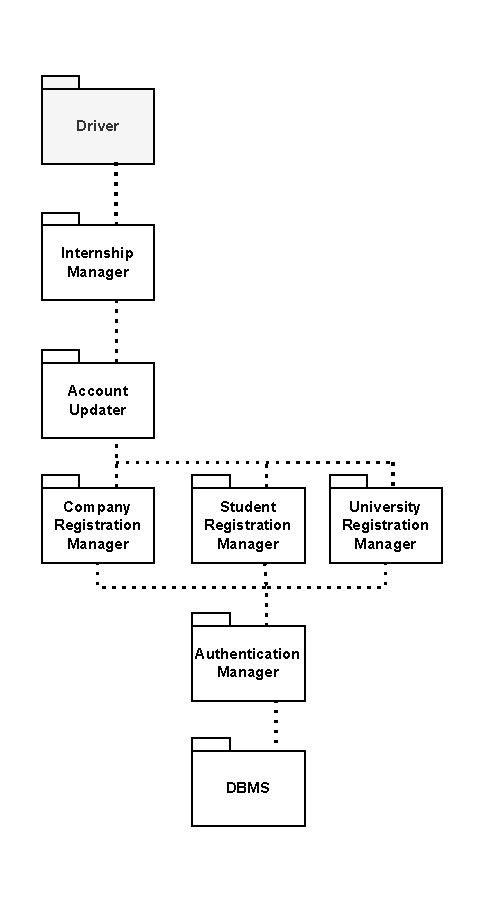
\includegraphics[width=0.5\linewidth]{DD/Images/Testing/5_Internship.drawio.pdf}
    \caption{Integration 5: Internship Manager.}
    \label{fig:integration_5}
\end{figure}

The Internship Manager builds upon user profiles created by the Account Manager. Its functionalities depend on a stable database and user registration system.
\newpage
    \item 
\textbf{Enhance and Recommendation Services:} \\
The Enhance Manager and Recommendation Manager can be developed in parallel, as they operate independently but rely on the same underlying data structures.

\begin{figure}[H]
    \centering
    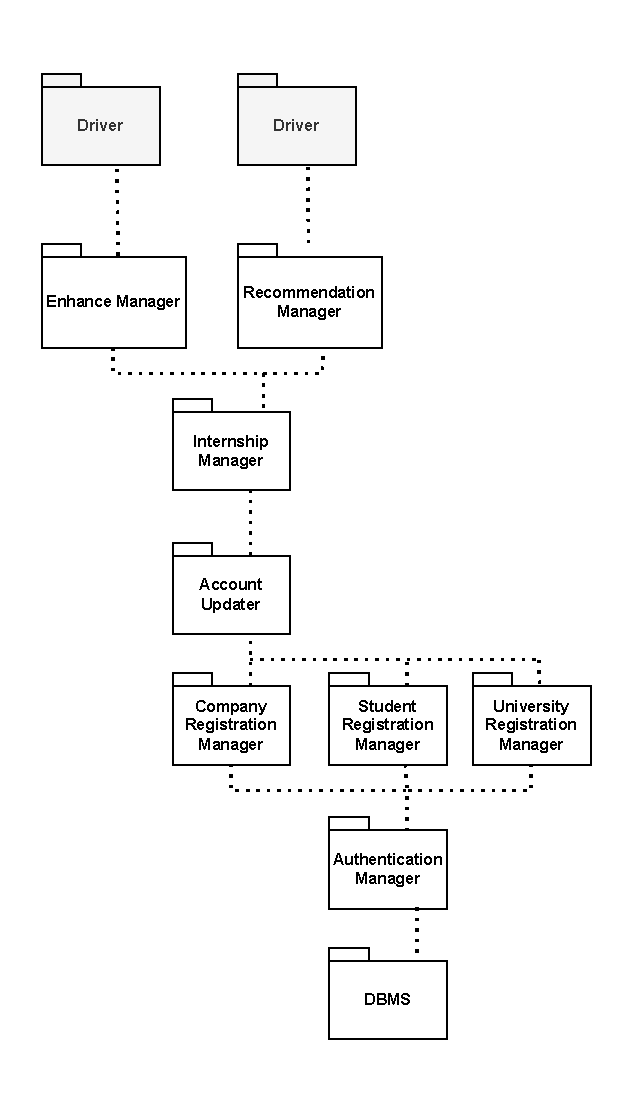
\includegraphics[width=0.5\linewidth]{DD/Images/Testing/6_EnhanceRec.drawio.pdf}
    \caption{Integration 6: Enhance and Recommendation Services.}
    \label{fig:integration_6}
\end{figure}

These services leverage data generated by the Internship Manager and Account Manager. Their modular nature allows simultaneous development.
\newpage
    \item 
\textbf{User Interactions (Chat and Report Manager):} \\
The Chat Manager and Report Manager facilitate user interactions.

\begin{figure}[H]
    \centering
    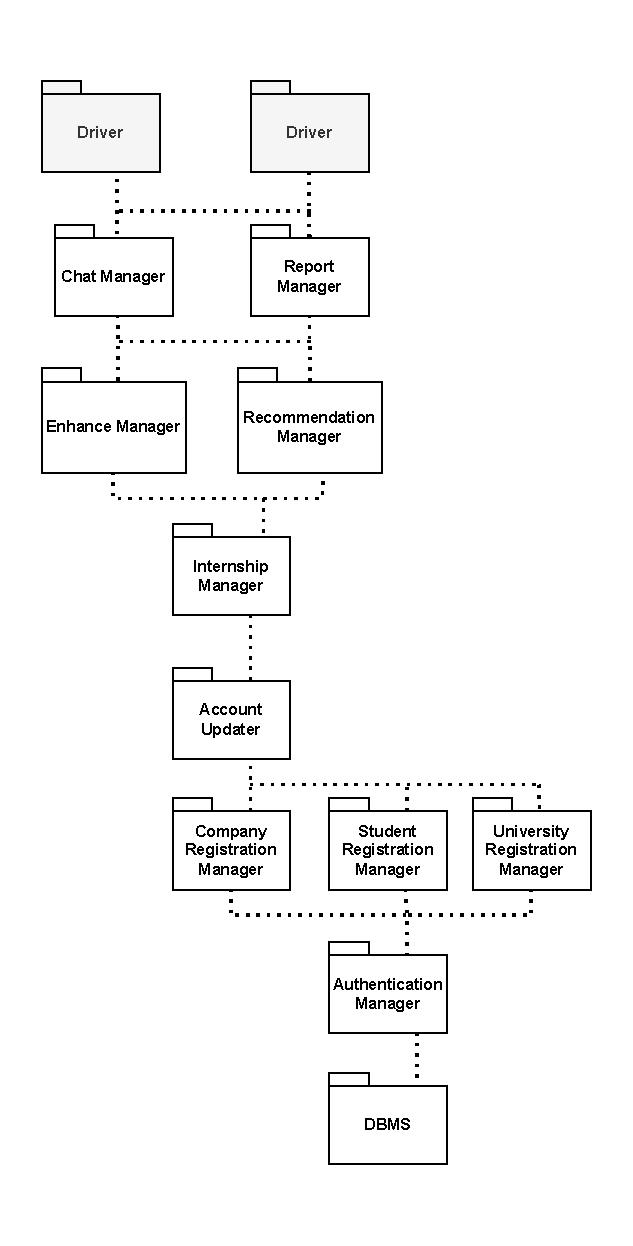
\includegraphics[width=0.5\linewidth]{DD/Images/Testing/7_ChatRep.drawio.pdf}
    \caption{Integration 7: Chat and Report Manager.}
    \label{fig:integration_7}
\end{figure}

These components rely on the existence of users, internships, and a communication infrastructure.
\newpage
    \item 
\textbf{Event Management Services (Notification and Calendar Manager):} \\
The final step includes the Notification Manager and the Calendar Manager, as both depend on events generated by other components.

\begin{figure}[H]
    \centering
    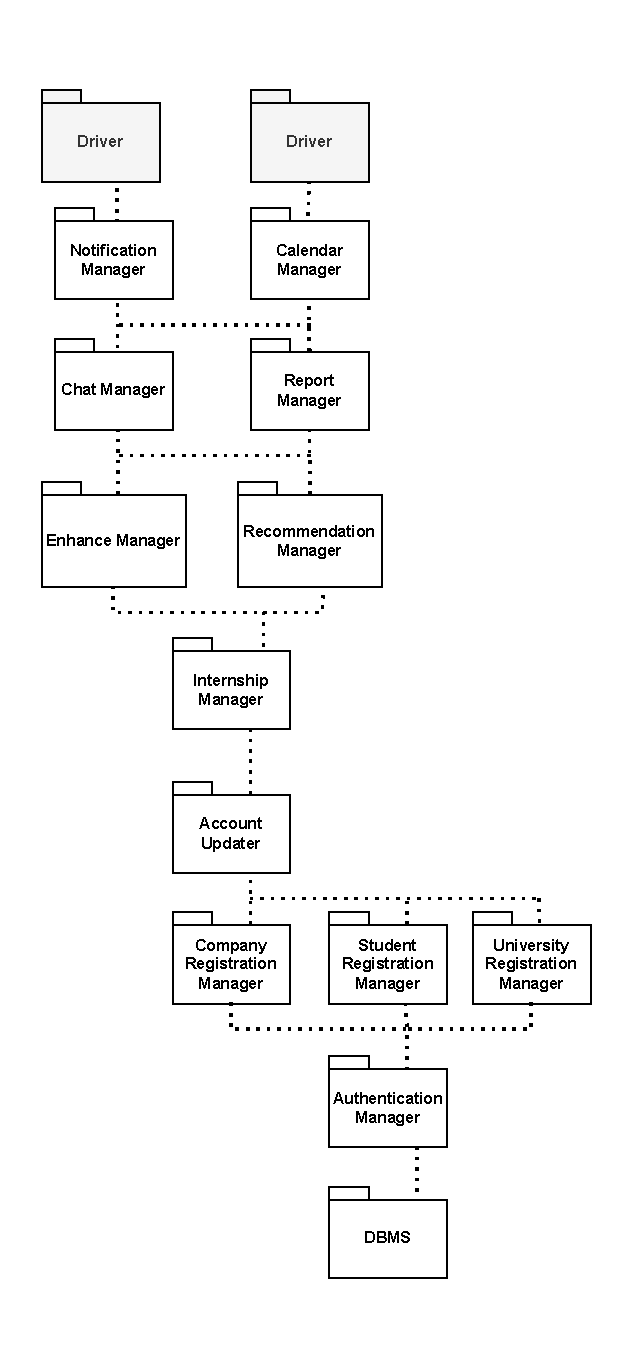
\includegraphics[width=0.5\linewidth]{DD/Images/Testing/8_NotCal.drawio.pdf}
    \caption{Integration 8: Notification and Calendar Manager.}
    \label{fig:integration_8}
\end{figure}

Both the Notification Manager and Calendar Manager are crucial for managing user events and enhancing overall system usability. They are implemented last to ensure all triggering events are in place and functional.
\end{enumerate}

\section{System Testing Plan}

Once all system components have been integrated, System Testing begins. System Testing ensures all modules function cohesively and meet requirements. The process includes:

\begin{itemize}
    \item 
\textbf{Unit Testing} \\
Each sub component undergoes isolated and specific testing using mock data.
    \item
\textbf{Integration Testing} \\
Test interactions between modules (e.g., data flow from the Enhance Manager to the Notification Manager).
    \item
\textbf{Functional Testing} \\
Verify that requirements, use cases and specifications previously described are properly satisfied.
    \item
\textbf{Performance Testing} \\
Evaluate the system's scalability under high traffic conditions to identify and address performance bottlenecks. The primary objective is to optimize the application's response time, resource utilization, and throughput, ensuring smooth operation and user satisfaction during peak usage periods.
\end{itemize}